%% Included in decks: slidemage-manual
%%

% SlideMage manual, chapter "Working in SlideMage": the deck editor, showing
% this manual's own deck (tools/manual/make_screenshots.py).
\begin{standardframe}{The deck editor}
	{\setlength{\fboxsep}{0pt}\fcolorbox{c_primary_gray}{white}{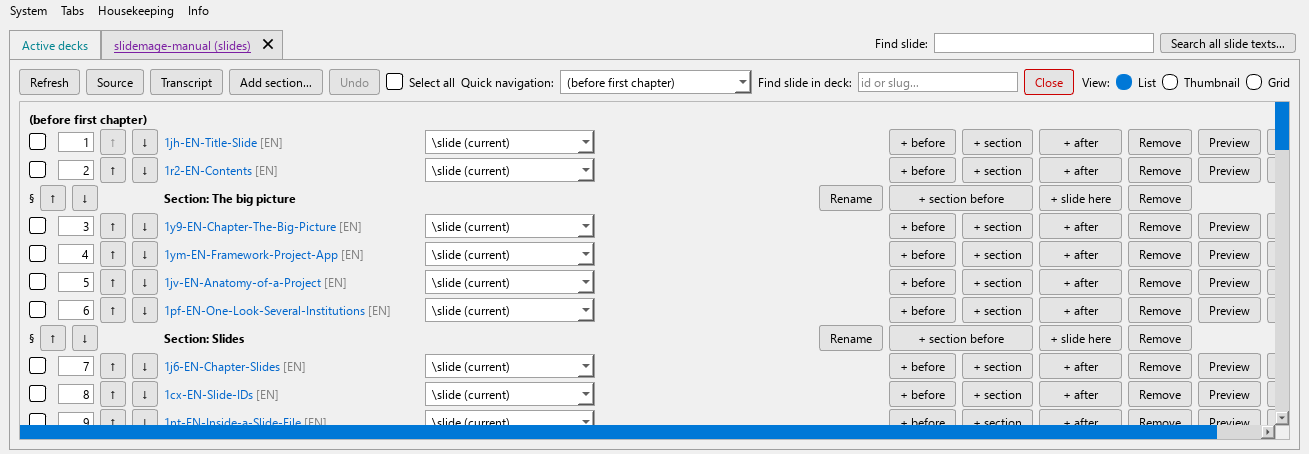
\includegraphics[width=0.66\linewidth]{media/screenshot-slidemage-deck-editor-list.png}}}\par\medskip
	\begin{columns}[t,onlytextwidth]
		\begin{column}{0.48\linewidth}
			\shrinklists{1}
			\begin{itemize}
				\item A deck's slides and chapters as rows; views \emph{List}, \emph{Thumbnail}, \emph{Grid}
				\item \emph{+ before} / \emph{+ after}: the \emph{Add slide} dialog -- create a new slide, use an existing one, or duplicate one
			\end{itemize}
		\end{column}
		\begin{column}{0.48\linewidth}
			\shrinklists{1}
			\begin{itemize}
				\item The dropdown chooses how the slide is included (\SMCmd{slide}, \SMCmd{slidestep}, \ldots)
				\item Move a slide by typing its new number; chapters: add, rename, move; \emph{Undo}
			\end{itemize}
		\end{column}
	\end{columns}
\end{standardframe}
